%; whizzy chapter -dvi
% -initex iniptex -latex platex -format platex -bibtex jbibtex -fmt fmt
% 以上 whizzytex を使用する場合の設定。
 
%     Tokyo Debian Meeting resources
%     Copyright (C) 2012 Junichi Uekawa
%     Copyright (C) 2011, 2015 Nobuhiro Iwamatsu

%     This program is free software; you can redistribute it and/or modify
%     it under the terms of the GNU General Public License as published by
%     the Free Software Foundation; either version 2 of the License, or
%     (at your option) any later version.

%     This program is distributed in the hope that it will be useful,
%     but WITHOUT ANY WARRANTY; without even the implied warranty of
%     MERCHANTABILITY or FITNESS FOR A PARTICULAR PURPOSE.  See the
%     GNU General Public License for more details.

%     You should have received a copy of the GNU General Public License
%     along with this program; if not, write to the Free Software
%     Foundation, Inc., 51 Franklin St, Fifth Floor, Boston, MA  02110-1301 USA

%  preview (shell-command (concat "evince " (replace-regexp-in-string "tex$" "pdf"(buffer-file-name)) "&"))

%%ここからヘッダ開始。

\documentclass[mingoth,a4paper]{jsarticle}
\usepackage{monthlyreport}
% 日付を定義する、毎月変わります。
\newcommand{\debmtgyear}{2015}
\newcommand{\debmtgmonth}{7}
\newcommand{\debmtgdate}{25}
% started from zero:
% (let ((year 2013) (month 7)) (+ (* (- year 2005) 12) month -1))
\newcommand{\debmtgnumber}{128}

\begin{document}

\begin{titlepage}
\thispagestyle{empty}
% タイトルページ:編集必要な部分は最初のマクロに飛ばすこと

\vspace*{-2cm}
第\debmtgnumber{}回 東京エリア Debian 勉強会資料\\
\hspace*{-2cm}

\includegraphics{image2012-natsu/dotdeb.pdf}\\
\hfill{}\debmtgyear{}年\debmtgmonth{}月\debmtgdate{}日

% ここはアップデートすること
% 全角文字にしないとフォントのサイズが合わないので注意
\rotatebox{10}{\fontsize{30}{30} {\gt 特集:DebianでHTTP/2を試す}}\\

\vspace*{-2cm}
\hfill{}
\includegraphics[height=6cm]{image200502/openlogo-nd.eps}
\end{titlepage}

\newpage

\begin{minipage}[b]{0.2\hsize}
 \definecolor{titleback}{gray}{0.9}
 \colorbox{titleback}{\rotatebox{90}{\fontsize{80}{80} {\gt デビアン勉強会} }}
\end{minipage}
\begin{minipage}[b]{0.8\hsize}
\hrule
\vspace{2mm}
\hrule
\begin{multicols}{2}
\tableofcontents
\end{multicols}
\vspace{2mm}
\hrule
\end{minipage}

\dancersection{事前課題}{野島 貴英}

今回の事前課題は以下です:
\begin{enumerate}
\item 本日、何の作業をやるかを宣言ください。
\item (オプション) どこで今回の勉強会の開催を知りましたか?
\item (オプション) 何について聞きたい/参加者と話をしたいですか?
\end{enumerate}
この課題に対して提出いただいた内容は以下です。
\begin{multicols}{2}
{\small
\begin{prework}{ $BLnEg(B }
  \begin{enumerate}
  \item Q.hack time$B$K2?$r$7$^$9$+!)(B\\
    A. $B@-D($j$b$J$/(BNook HD+$B$N(BDebian$B2=!#(B
  \item ($B%*%W%7%g%s(B)Q.$B2?$K$D$$$FJ9$-$?$$!?;22C<T$HOC$r$7$?$$$G$9$+!)(B\\
    A. $B2F5Y$_$K(BDebian$B$G2?$r$9$k!*!)(B
  \end{enumerate}
\end{prework}

\begin{prework}{ issei }
  \begin{enumerate}
  \item Q.hack time$B$K2?$r$7$^$9$+!)(B\\
    A. Hurd$B$r%$%s%9%H!<%k(B
  \end{enumerate}
\end{prework}

\begin{prework}{ wskoka }
  \begin{enumerate}
  \item Q.hack time$B$K2?$r$7$^$9$+!)(B\\
    A. tilegx$B$X$N0\?"(B
  \item ($B%*%W%7%g%s(B)Q.$B$I$3$G:#2s$NJY6/2q$N3+:E$rCN$j$^$7$?$+!)(B\\
    A. $B$=$NB>(B
  \end{enumerate}
\end{prework}

\begin{prework}{ dictoss }
  \begin{enumerate}
  \item Q.hack time$B$K2?$r$7$^$9$+!)(B\\
    A. jessie$B$GF0:n3NG'MQ$N(Blxc$B%3%s%F%J$r:n$C$FF0$+$7$F$_$k(B
  \item ($B%*%W%7%g%s(B)Q.$B$I$3$G:#2s$NJY6/2q$N3+:E$rCN$j$^$7$?$+!)(B\\
    A. Twitter (\@debianjp)
  \end{enumerate}
\end{prework}

\begin{prework}{ nametake }
  \begin{enumerate}
  \item Q.hack time$B$K2?$r$7$^$9$+!)(B\\
    A. Debian$B4D6-9=C[(B
  \item ($B%*%W%7%g%s(B)Q.$B$I$3$G:#2s$NJY6/2q$N3+:E$rCN$j$^$7$?$+!)(B\\
    A. $B$=$NB>(B
  \end{enumerate}
\end{prework}

\begin{prework}{yy\_y\_ja\_jp}
  \begin{enumerate}
  \item Q.hack time$B$K2?$r$7$^$9$+!)(B\\
    A. DDTSS
  \item ($B%*%W%7%g%s(B)Q.$B2?$K$D$$$FJ9$-$?$$!?;22C<T$HOC$r$7$?$$$G$9$+!)(B\\
    A. DDTSS
  \end{enumerate}
\end{prework}

\begin{prework}{koedoyoshida}
  \begin{enumerate}
  \item Q.hack time$B$K2?$r$7$^$9$+!)(B\\
    A. $B$"$s$I$-$e$a$s$F$C$I$G$S$"$sJT=8(B
  \item ($B%*%W%7%g%s(B)Q.$B$I$3$G:#2s$NJY6/2q$N3+:E$rCN$j$^$7$?$+!)(B\\
    A. $B$=$NB>(B
  \end{enumerate}
\end{prework}


}
\end{multicols}

\dancersection{Debian Trivia Quiz}{野島 貴英}

 Debianの昨今の話題についてのQuizです。

今回の出題範囲は\url{debian-devel-announce@lists.debian.org} や \url{debian-news@lists.debian.org}に投稿された
内容などからです。

\begin{multicols}{2}
%; whizzy-master ../debianmeetingresume201311.tex
% $B0J>e$N@_Dj$r$7$F$$$k$?$a!"$3$N%U%!%$%k$G(B M-x whizzytex $B$9$k$H!"(Bwhizzytex$B$,MxMQ$G$-$^$9!#(B
%

\santaku
{6/22$B$K$F!"(Bbackport$B$N%A!<%`$,!"FCDj$N>r7o$rK~$?$9%Q%C%1!<%8$r$4$C$=$j>C$7$?$N$O!"$I$N(Bbackports?}
{squeeze-backports}
{wheezy-backports}
{jessie-backports}
{B}
{jessie$B$GMxMQ$G$-$J$$%Q%C%1!<%8$r!"(Bwheezy-backports$B$+$i$4$C$=$j>C$7$?$H$N$3$H$G$9!#(Bbackports$B$K4^$^$l$k$I$N%Q%C%1!<%8$,$I$&$J$C$F$$$k$+!)$I$&$7$FM_$7$$$+!)$K$D$$$F$O!"(Bfreeze$B$N4|4V$H(Bfreeze$B8e$N$o$:$+$J4|4V$N4V$K!"(Bbackport$BC4Ev$+$i(Bbackports$B%A!<%`$K<+H/E*$K%?%$%`%j!<$KAjCL$7$FMh$FM_$7$$$H$N4+9p$b9T$o$l$^$7$?!#(B}

\santaku
{7/7$B$K$F!"(Bsid$B$G$O!"FCDj%P!<%8%g%s$N(BGCC$B$H(Blibstdc++$B$G%3%s%Q%$%k!&F0:n=PMh$k$h$&$K$7$FM_$7$$;]$N%"%J%&%s%9$,N.$l$^$7$?!#$I$NAH$_9g$o$;!)(B}
{gcc 6/libstdc++6}
{gcc 4/libstdc++5}
{gcc 5/libstdc++6}
{C}
{$B$^$:$O!"(BDebian sid$B$G$O!"(Bgcc 5/libstdc++6$B$G%3%s%Q%$%k!&F0:n=PMh$k$h$&$K%Q%C%1!<%8%a%s%F%J$NJ}$O=$@5BP1~$r$7$FM_$7$$;]$N%"%J%&%s%9$,$"$j$^$7$?!#:#2s!"(BABI$B%Y!<%9$G$bJQ99$K$J$C$?$j!"(BC++11$B$KBP1~$H$J$C$?$j$G1F6A$,=t!9H/@8$7$^$9!#$^$?!"$3$N1F6A$G!"(BGFortran$BB&$b(Bmodule 14$B$X0\9T$H$J$k$N$G!"(BGFortran$B$r;H$C$F$$$k%Q%C%1!<%8%a%s%F%J$bBP1~$,I,MW$H$N$3$H$G$9!#(B}

\santaku
{7/8$B$K$F!"J#?t$N(Bupstream$B$+$iDs6!$5$l$F$$$k(Blibav*$B72$N%i%$%V%i%j$K$D$$$F!"Ds6!85$N(Bupstream$B$rJQ99$9$k$H$NO"Mm$,$"$j$^$7$?!#$I$N(Bupstream$B$KJQ99$H$J$C$?$N$G$7$g$&$+!)(B}
{FFmpeg}
{libav.org}
{VideoLAN}
{A}
{libav*$B$H$$$&%^%k%A%a%G%#%"$N%G!<%?$r07$&%i%$%V%i%j$J$N$G$9$,!"0lC6(Blibav.org$B$,Ds6!$7$F$$$k$b$N$KJQ99$H$J$C$?$N$G$9$,!"$^$?(BFFmpeg$B$,Ds6!$7$F$$$k$b$N$KLa$C$F$-$?>u67$G$9!#5DO@$N%5%^%j$O(B https://wiki.debian.org/Debate/libav-provider/ffmpeg}

\santaku
{DPL$B$N(BNeil MacGovern$B$,(Breddit$B$K3+$$$?!V(BDPL$B$@$1$I!"2?$+<ALd$"$k!)!W$H$$$&%9%l$G!"(BDPL$B$K$H$C$F$b@($$$H;W$&%G%#%9%H%j%S%e!<%7%g%s$H$7$F$"$2$i$l$F$?$b$N$O$I$l!)(B}
{$BEvA3(BDebian$B$C$7$g!*(B}
{ArchLinux}
{ubuntu}
{B}
{$B%9%l$N=;?M$N<ALd$K!"(BDPL$B$,(BArchLinux$B$,@($$$HEz$($F$$$^$7$?!#(Bwiki$B$N=<<B$V$j$,$H$K$+$/AG@2$i$7$$$H$N$3$H!#(B}

\santaku
{7/20$B$K(Bdgit$B$N?7$7$$%P!<%8%g%s$N$b$N$,%j%j!<%9$5$l$^$7$?!#$I$N%P!<%8%g%s$K$J$C$?!)(B}
{0.1}
{0.3}
{1.0}
{C}
{Debian$B%"!<%+%$%V$r(Bgit$B$GA`:n$G$-$k%D!<%k$N(Bdgit$B$,(B1.0$B$,%j%j!<%9$5$l$?$H$N$3$H$G$9!#AaB.(Bdebian sid$B$K<}O?$5$l$F$$$^$9!#(Bdgit clone package$BL>$H$9$k$H!"(Bhttps://git.dgit.debian.org/ $B$G4IM}$5$l$F$$$k$b$N$,<j85$K(Bclone$B$5$l$^$9!#(B}

\santaku
{7/21$B$K(B Debian Installer Stretch Alpha 1$B$,%j%j!<%9$5$l$^$7$?!#JQ99E@$O0J2<$N$I$l!)(B}
{UEFI$B%V!<%H$rEk:\(B}
{$B%M%C%H%o!<%/(BIF$B$,(BMAC$B%"%I%l%9$K$J$k(B}
{$B%$%s%9%H!<%k;~$N(BUI$B$,(Btext$B%b!<%I$+$i(Bgraphical$B%b!<%I$K$J$C$?(B}
{C}
{Strech$B$GMxMQ$5$l$k$G$"$m$&!"%$%s%9%H!<%i%W%m%0%i%`$N&A(B1$B$,%j%j!<%9$5$l$^$7$?!#$b$A$m$s!"(BStrech$B$,%j%j!<%9$5$l$?$o$1$G$O$J$$$N$GCm0U!#JQ99E@$O?t!9$"$j!"%G%U%)%k%H$N(BCPU$B%"!<%-%F%/%A%c$,(Bamd64$B$K$J$C$?$j$7$?!#>\$7$/$O(Bdebian-devel-announce$B$r;2>H(B}

\end{multicols}

\dancersection{最近のDebian関連のミーティング報告}{野島 貴英}

\subsection{第127回東京エリアDebian勉強会}

\begin{itemize}
\item 場所はスクウェア・エニックスさんのセミナルームをお借りしての開催でした。
\item 参加者は6名でした。
\item セミナ内容は野島さんによる「Debianと脆弱性対応のあれこれ」でした。
\item 残りの時間でhack timeを行い、成果発表をしました。
\item 宴会の代わりに、「まいどおおきに食堂」で夕食会をやりました。
\end{itemize} 

  セミナは野島さんより、Debianと脆弱性対応について諸々発表がありました。内容としては、すでに公開されている昨今の件のサマリとなりましたが、会場ではいろいろ議論や、追加の情報をいただくことが出来非常に有意義でした。
  
  元々、本発表は別で開かれたクローズドなセキュリティの勉強会で発表する用に作ったものではありますが、改めてまとめて見るといろいろ気づく事があり、新鮮でした。debianのセキュリティチームからCVE、他のディストリビューションまでOSSの脆弱性の連絡体制ができているのは、さすが沢山の人に支えられているディストリビューションなだけあると思います。

% % (query-replace-regexp "<.*?>" "")
% % (query-replace-regexp "^[	 ]\+" "")

%-------------------------------------------------------------------------------
\dancersection{DebianでHTTP/2を試す}{野島 貴英}
%-------------------------------------------------------------------------------

\subsection{はじめに}

 2015/5にHTTP/2がRFC7540として遂に文章化されました。また、最近でも、ほうぼうでWEBページあるいはサービスについて、HTTP/2の対応度合いについて聞かれるようになってきました\footnote{某有名携帯電話イベントでHTTP/2をアプリ開発者に全力推奨している件を見てマヂ慌てたりしたのは秘密...}。

 ここでは、Debianで、HTTP/2の環境をちょっと作って試してみました。

\subsection{ところでHTTP/2って?}

  WEBブラウザがサーバと通信する際に、HTTP/1.x(xは0,1の数字)が長年(HTTP/1.1は15年以上も!)使われています。しかしながら、昨今のWEBページは、HTTP/1.xが策定された頃に比べて格段にリッチなページとなっており、1ページを表示する為に必要な通信量は格段に増えています。HTTP/1.xのままでは、WEBの通信が非効率となってしまいました。

 HTTP/1.1の欠点を克服するために、google社でSPDYが開発され、さらにSPDYを参考にして、沢山の人の貢献により、次世代のHTTP通信規格が策定されました。これがHTTP/2となります。

 \subsection{HTTP/2の特徴}

 HTTP/2の特徴としては以下の通りです\cite{ref:http-2-faq}。
 
\begin{itemize}
\item テキスト電文ベースではなく、バイナリ電文を使います。
\item 1本のTCPコネクション上で、複数のリクエスト・レスポンスを多重化してやりとりできるように設計されています。
\item  リクエスト・レスポンスに使われるヘッダ情報を無駄の無い電文にし、さらに圧縮し、より効率的に通信できるようにしています。実はモバイル端末などでは、パケットの往復にかかる時間が長いので、リクエスト・レスポンスの開始1パケット目にできるだけ情報を詰め込むことは通信時間を縮めるのに非常に有効です。
\item 1つのリクエストで、ブラウザが続けて必要とするデータをまとめてレスポンスできる機能が入りました(サーバプッシュという機能。)\cite{ref:server-push-primer}
 \end{itemize}

\subsection{HTTP/2さらに詳しく}

  これ以上HTTP/2プロトコルについて、詳しく調べたい人は、

 \begin{itemize}
  \item HTTP/2本家\\
    \url{https://http2.github.io/}
  \item 高速・大規模ネットワーク時代に向けて改良されたHTTP/2プロトコル
    \url{http://www.atmarkit.co.jp/ait/articles/1409/18/news135.html}
  \item twitterの\#http2studyタグ
  \item http/2 Advent Calender 2014
    \url{http://qiita.com/advent-calendar/2014/http2}
\end{itemize}

 などなど、多数の良い解説がありますので是非ご覧ください。これ以上細かいHTTP/2のプロトコル仕様についてはここでは割愛します。

 \subsection{HTTP/2の良いデモサイト}

 論より証拠で、HTTP/2が優れているか?を試せる非常に良いデモサイトがあります。是非お試し下さい。なお、Debian sidのchromium/iceweaselで動作確認を確認できています。
 \\
\begin{center} 
 \url{https://http2.golang.org/gophertiles}
\end{center}

\subsection{HTTP/2の通信開始の仕方}

 HTTP/2を使ってブラウザからアクセスするとき、現状、TLSのALPN/NPNでHTTP/2を指定して、やりとりを開始するやり方しか現行ブラウザには実装されていません。というわけで、事実上、HTTP/2のサイトは、全部フルSSL化されている状況となります\cite{ref:wikipedia-http-2}。

 一方、TLSを使わない場合、HTTP/1.1のリクエストヘッダに特別なヘッダを混ぜることにより、HTTP/2へアップグレードして、以降HTTP/2でやり取りをするという手法があります。しかしながら、こちらはブラウザが対応していません\cite{ref:http-2-protocol-upgrade-primer}。

\subsection{DebianでHTTP/2をお手軽に楽しむ}

 HTTP/2をDebianでお手軽に楽しむには以下の環境を用意します。

 \begin{itemize}
  \item クライアント側準備\\
    chromiumか、iceweasel
  \item サーバー側準備\\
     nghttp2,Apache Traffic Server等など
 \end{itemize}  
 
 \subsection{クライアント側準備}

 以下にchromiumと、iceweaselについて、HTTP/2用を評価するのに便利なセットアップについて載せます。

 \subsubsection{chromium}

 chromiumを使う場合は次の通りです。まず、Debianにchromiumブラウザを導入します。
  
\begin{commandline}
$ sudo apt-get install chromium
\end{commandline}
% $
次に、chromiumを起動して左隅みに現れる「Apps」$\rightarrow$「Web Store」をアクセスし、「HTTP/2 and SPDY indicator」を導入してください。

 以上の操作を行ったchromiumでHTTP/2対応のサイトにアクセスすると、青い稲妻マークがアドレスバーに表示されるようになります。

\begin{figure}[H]
\begin{center}
 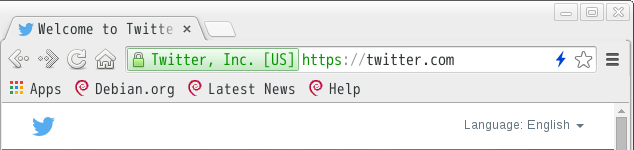
\includegraphics[width=0.9\hsize]{image201507/chromium-http-2-ready.png}
\end{center}
\caption{chromiumでHTTP/2のサイトにアクセス}
\end{figure}

\subsubsection{iceweasel}

 iceweaselを使う場合は次の通りです。まず、iceweaselと、xul-ext-spdy-indicatorをDebianに導入します。
  
\begin{commandline}
$ sudo apt-get install iceweasel xul-ext-spdy-indicator
\end{commandline}
% $

以上の操作を行ったiceweaselでHTTP/2対応のサイトにアクセスすると、青い稲妻マークがアドレスバーに表示されるようになります。

\begin{figure}[H]
\begin{center}
 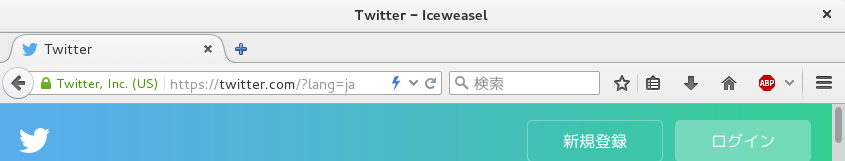
\includegraphics[width=0.9\hsize]{image201507/iceweasel-http-2-ready.png}
\end{center}
\caption{iceweaselでHTTP/2のサイトにアクセス}
\end{figure}

\subsection{サーバ側準備}

 いよいよDebianにサーバ側を準備します。

\subsubsection{HTTP/2に対応しているサーバ}

 どんなサーバがHTTP/2に対応しているかは、\\
\\
 Implementations \\
  \url{https://github.com/http2/http2-spec/wiki/Implementations}\\
\\
 を参照ください。

\subsubsection{nghttp2パッケージ}

 Debian sidにて、HTTP/2対応サーバのパッケージとして、nghttp2があります。ここではこちらを使ってサーバを作ることにします。

 \begin{commandline}
$ sudo apt-get install nghttp2 ssl-cert
\end{commandline}
% $

 なお、閲覧可能なコンテンツとして、groffの付属htmlマニュアルをドキュメントルートにしたHTTP/2サーバを立ててみます。

  なお、*-snakeoil.*というファイルは、ssl-crtパッケージを導入すると勝手に作成される自己証明書ファイルとなります。
  
\begin{commandline}
$ sudo nghttpd -D -d /usr/share/doc/groff-base/html/ \
  443 /etc/ssl/private/ssl-cert-snakeoil.key \
  /etc/ssl/certs/ssl-cert-snakeoil.pem
\end{commandline}  
%$

\subsection{アクセスしてみる}

  ブラウザで、アクセスしてみます。\\
 アクセス先:\url{https://localhost/pic-6.html}

 chromium/iceweasel共に無事にHTTP/2対応を示す青い稲妻マークがURL表示部分に付いていることが判ります。

\begin{minipage}{0.5\hsize}
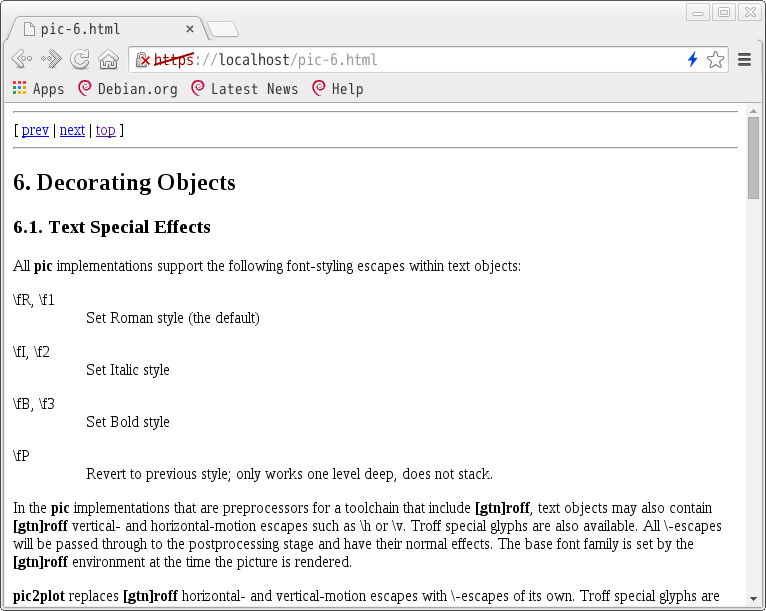
\includegraphics[width=0.9\hsize]{image201507/chromium-groff-access.png}
\end{minipage}
\begin{minipage}{0.5\hsize}
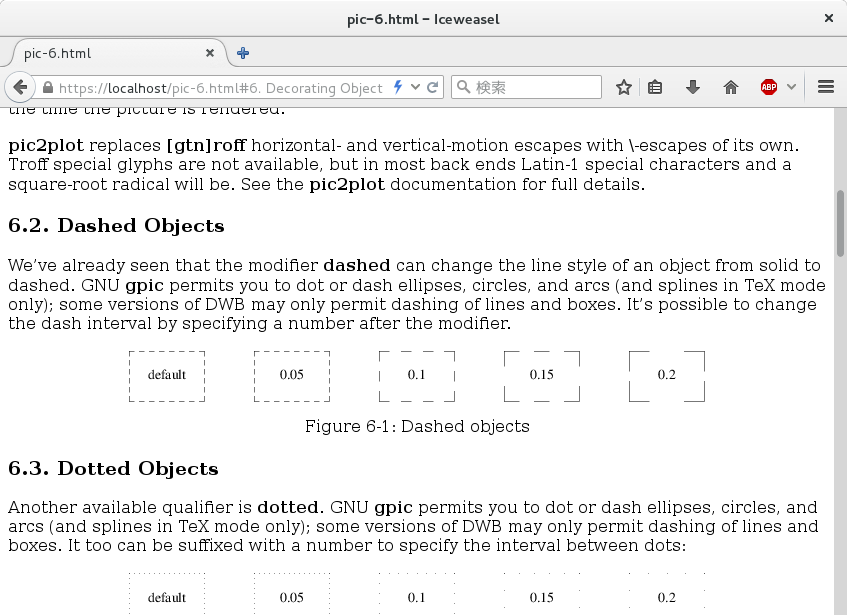
\includegraphics[width=0.9\hsize]{image201507/iceweasel-groff-access.png}
\end{minipage}
 
\subsection{proxyサーバで既存サイトのHTTP/2化をやってみる}

 さて、nghttpdは軽量のHTTP/2対応WEBサーバではあるのですが、やっぱりapacheのような高機能なWEBサーバを使ってHTTP/2を実現したいというニーズがあると思います。(例:phpのサイトをHTTP/2化したい等)

 今度は、apacheをバックエンドにして、nghttp2付属のproxyサーバを使い、サイトのHTTP/2化を行ってみます。
  
 今回用意しようとしている環境の概念図を載せます。

\begin{figure}[H]
\begin{center}
 \includegraphics[width=0.5\hsize]{image201507/nghttpx-apache-proxying.eps}
\end{center}
\caption{proxyサーバでHTTP/2化を行う環境の概念図}
\end{figure}
  
 proxyとapacheの環境をDebianに用意します。手順は次の通りです。

\begin{description}
\item [Step 1.] sudo apt-get install apache2 nghttp2 ssl-cert
\item [Step 2.] sudo a2enmod userdir
\item [Step 3.] cd /home/yours/; mkdir public\_html
\item [Step 4.] cd public\_html; cp -a /usr/share/doc/groff-base/html .
\item [Step 5.] sudo vi /etc/nghttpx/nghttpx.conf\\
\begin{commandline}
 ----nghttpx.confの中身ここから----
frontend=0.0.0.0,443 
backend=127.0.0.1,80 
private-key-file=/etc/ssl/private/ssl-cert-snakeoil.key 
certificate-file=/etc/ssl/certs/ssl-cert-snakeoil.pem 
workers=1 
----ここまで----
\end{commandline}
\item [Step 6.] sudo systemctl start apache2.service
\item [Step 7.] sudo nghttpx -D --conf /etc/nghttpx/nghttpx.conf
\end{description}

 以上できましたら、いよいよ先に用意したブラウザからアクセスしてみます。無事 apache側に用意したサイトが、HTTP/2対応できている事がわかります。\\
\\
 アクセス先:\url{http://localhost/~yours/html/pic.html}\\

\subsection{おわりに}

  HTTP/2もDebianを使えば簡単に実験できます。また、沢山のファイルで構成されるページがあると、HTTP/2は非常に威力を発揮します。この機会にHTTP/2を是非お試し頂き、その威力を確認してみてください。
  
\begin{thebibliography}{9}
\bibitem{ref:http-2-faq} HTTP/2 Frequently Asked Questions,\url{https://http2.github.io/faq/}
\bibitem{ref:server-push-primer} 初めてのHTTP/2サーバプッシュ,\url{http://labs.gree.jp/blog/2014/12/11987/}
\bibitem{ref:wikipedia-http-2} wikipedia HTTP/2の章,\url{https://ja.wikipedia.org/wiki/HTTP/2}
\bibitem{ref:http-2-protocol-upgrade-primer} HTTP/2 プロトコルネゴシエーション方法と ATS での実装,\url{http://techblog.yahoo.co.jp/infrastructure/http2/ats_http2_pn/}
\end{thebibliography}
   
%-------------------------------------------------------------------------------
\dancersection{会場での無線LANのつなぎ方}{野島 貴英,Roger}
%-------------------------------------------------------------------------------
 \subsection{はじめに}

 今回試験として、会場側でフィルタ無しのグローバル回線を用意しました。
ただ、会場側のセキュリティポリシーにより、wpa-psk AES hidden SSIDという
方式での提供となります。

 以下にDebianマシンでの接続方法を記載します。

 また、自分の環境では違うやり方でつながったという方は、野島まで
教えて下さい。こちらでもノウハウとして溜めていく予定です。

 \subsection{wpasupplicant及び/etc/network/interfacesを利用の場合}

 もっとも良いマニュアルは、/usr/share/doc/wpasupplicant/README.Debian.gz
となります。困った場合はこちらも合わせてご参照下さい。

 以下に/etc/network/interfacesの定義について会場の例を記載します。

\begin{commandline}
$ sudo vi /etc/network/interfaces
-----以下のエントリがなければ追記ここから----------
iface wlan0_debian inet dhcp
     wpa-conf /etc/wpa_supplicant/wpa_supplicant_debian.conf
-----以下のエントリがなければ追記ここまで----------
$ sudo vi /etc/wpa_supplicant/wpa_supplicant_debian.conf
-----以下のエントリを追記ここから----------
network={
     ssid=<<会場のSSID>>
     psk=<<会場のパスワード>>
     scan_ssid=1
}
-----以下のエントリを追記ここまで----------
$ sudo chmod 600 /etc/wpa_supplicant/wpa_supplicant_debian.conf
$ sudo ifup wlan0=wlan0_debian
\end{commandline}
%$

 また、ハマってしまった時のデバッグ方法は、
/usr/share/doc/wpasupplicant/README.Debian.gz中の''4. Trubleshooting''の章が便利です。

 \subsection{その他の無線LAN用パッケージを利用の場合}

 すみません、自分が情報を持たないため、現場で教えて下さい。

\cleartooddpage

\vspace*{15cm}
\hrule
\vspace{2mm}

\includegraphics[width=2cm]{image200502/openlogo-nd.eps}
\noindent \Large \bf Debian 勉強会資料\\
\noindent \normalfont \debmtgyear{}年\debmtgmonth{}月\debmtgdate{}日 \hspace{5mm}  初版第1刷発行\\
\noindent \normalfont 東京エリア Debian 勉強会 (編集・印刷・発行)\\
\hrule

\end{document}
